% !TEX root = arbeit.tex
\section{Experiments}
% In zeitlicher Reihenfolgen auflisten, damit man sieht, zu welchem Zeitpunkt man mit welchen Teilen gearbeitet hat.
% In this section, all the different test (lab and simulations) are listed. As far as possible in their chronolocial order because between some lab tests there were simulations to improve the instrument before testing the redesigned instrument.

% Fügt ein PDF ein, nummeriert nach dem PDF normal weiter.
%\includepdf[pages=-]{Report_Thermofoil_UV_Masterarbeit.pdf}

	In this section , the different tests are described to develop the NIM instrument. All measurements were performed in the STROFIO vacuum chamber.
%------------------------------------------------------------------------------------
	\subsection{Reflectron}
	
	The NIM prototype reflectron was exchanged through the flight like reflectron, which was tested. The NIM prototype reflectron consisted of 12 ring electrodes connected with each other with resistors in between them. On the first, 5th and 12th electrode, a voltage can be applied. With the different resistors, a linear voltage gradient in the reflectron is generated.\\ % Noch besser formulieren.
	The flight reflectron consists of a ceramic tube with two resistance spirals on its inner walls. There are three electrodes, where the voltage can be applied. The electrodes are connected via resistance spirals with each other. The two reflectrons can be seen in Fig.\,\ref{fig:ExpRefl}. This kind of reflectron was also used in the RTOF mass spectrometer which flied in ROSINA \cite{Diss_Scherer} and the in the NGMS \cite{Diss_Hofer}. \\ % Evt. noch etwas schöner und weiter ausführen. Strahlungsfestigkeit musste getestet werden. Report? Paper? Diss?
	Therefore, the two reflectrons are from the electrical point of view the same.\\ % Oder kommt das erst bei der Auswertung?
	
	\begin{figure}[h]
		\begin{subfigure}{0.5\textwidth}
			\centering
			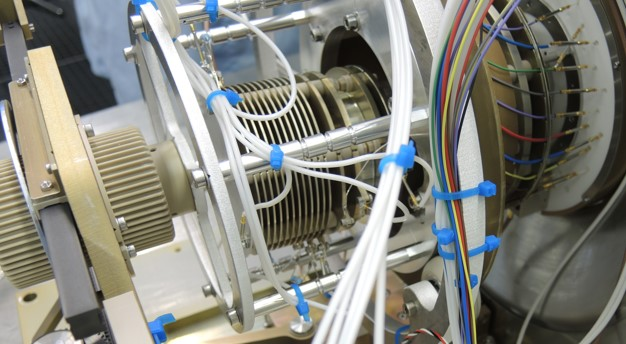
\includegraphics[width = 0.95\textwidth]{Bilder/reflectron_Prototype1.jpg}
		\end{subfigure}
		\begin{subfigure}{0.5\textwidth}
			\centering
			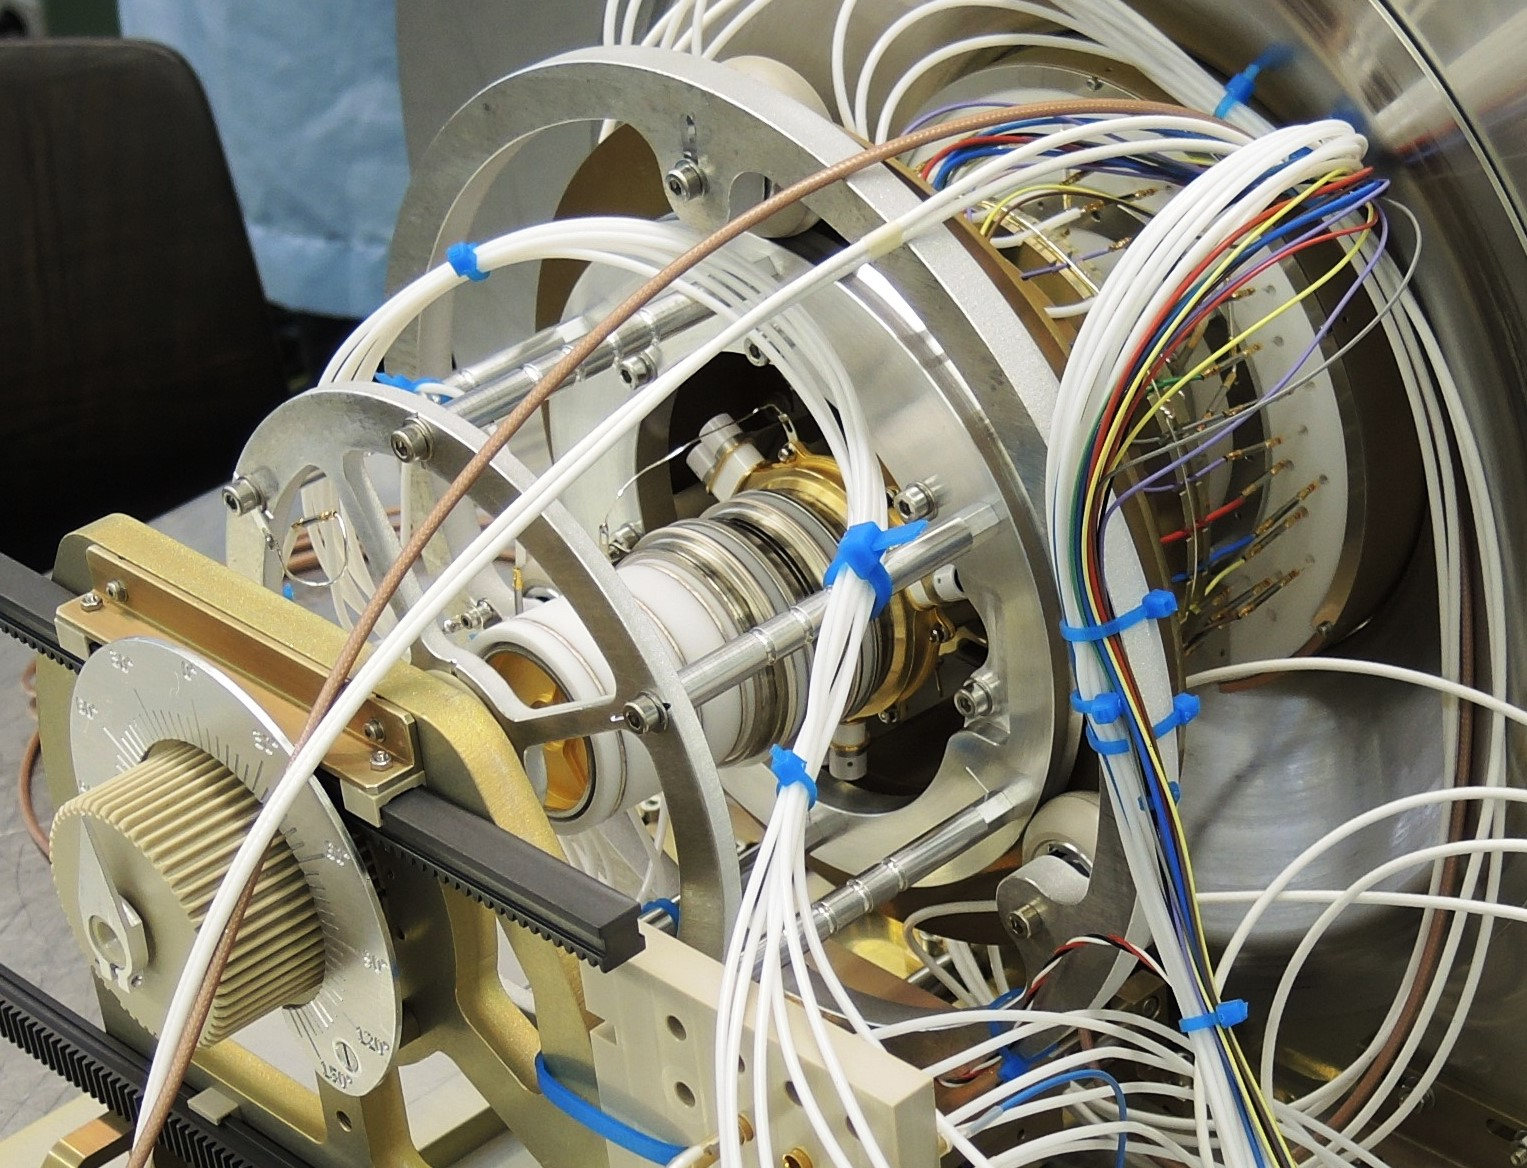
\includegraphics[width = 0.85\textwidth]{Bilder/reflectron_flight.JPG}
		\end{subfigure}
		\caption{Left: Prototype reflectron with ringelectrodes. Right: Flight reflectron}
		\label{fig:ExpRefl}
	\end{figure}

	\subsubsection{Measurement Principle}\label{subsec:ReflecMeasPric}
		% Vortrag Messbedingungen zusammenschreiben
	
	\subsubsection{Discussion}\label{subsec:ReflecDissc}
		% Graphiken neu machen. Achsenskalierung, Spannungssets-Vergleich? Nur sagen, dass sie beinahe identisch sind.
	
	
	% Messbedingungen. Eigenes kurzes Unterkapitel machen
	% Auswertung, eigenes kurzes Unterkapitel

	\begin{comment}
	
	Exchange of the reflectron. Messdaten und Auswertung. Spannungssets vergleichen. Vortrag zusammenschreiben. Plots von dort nehmen und noch etwas besser beschreiben.
	(Plot-Axis, enlarge the exponent of the 10^11 e-/ns)
		
		
		
		
		
	\end{comment}
	

	
	
		
	\subsection{CASYMIR-D/-E}
	% CASYMIR-D? Erst wenn man intensitätsproblem mit ante chamber gelöst hat :/. CASYMIR-E-Kampagne.
	
%-----------------------------------------------------------------------------------------
	\subsection{Simulations}
	% Evt. in einem eigenen Kapitel? Schauen, welchen Einfluss es dann jeweis auf die Hardware hatte. -> Elektronik setzt Spannungsranges, beschreiben, dass man da iterieren musste um das optimale Simulationsspannungsset zu finden mit den Grenzen, welche die Elektronik uns für die jeweiligen Elektroden gibt. -> vgl. mit den Messungen vom PFM.
	% Neusimulationen mit neuen Grenzen für die HV. -> die Resultate dieser Simulationen. Als Folgen davon wurden die Grenzen für die HV neu definiert. Schauen, wie man das am besten auseinander nimmt :/.

	% Pulsersimulationen -> Kriterien für Andy für das Pulserdesign. Ab wann wir einen Einbruch in der Massenauflösung haben. (Worddokument wo die einzelnen Bilder zusammengestellt sind?)
	
	
	
	% Filament repeller simulation tests. Noch Graphiken einmal einfügen. Die wichtigsten.
	% Um herauszufinden, wie wichtig die Position des Filaments ist.
	
	% Noch besser umschreiben. Die position des filaments entspricht nicht der erwarteten??? Was ist da schief gelaufen??? :(
	
	% Intensitätssimulation Countberechnung:
	% Man generiert 2000 e- auf dem Filament und zeichnet immer nach 1E-5 microsec auf, an welcher Position sich die Teilchen gerade befinden. Die Fkt. 'Plot_optVoltAndPos.m' zählt alle Positionen zusammen, welche sich in dem Zylindervolumen befinden. Die Grundfläche des Zylinders ist das Eintritts-Grid von der antechamber und die Höhe ist die Höhe der Entrance. Im th-Mode befinden sich nur in diesem Volumen neutrale Teilchen.
	\begin{figure}[h]
		\begin{subfigure}{0.53\textwidth}
			\centering
			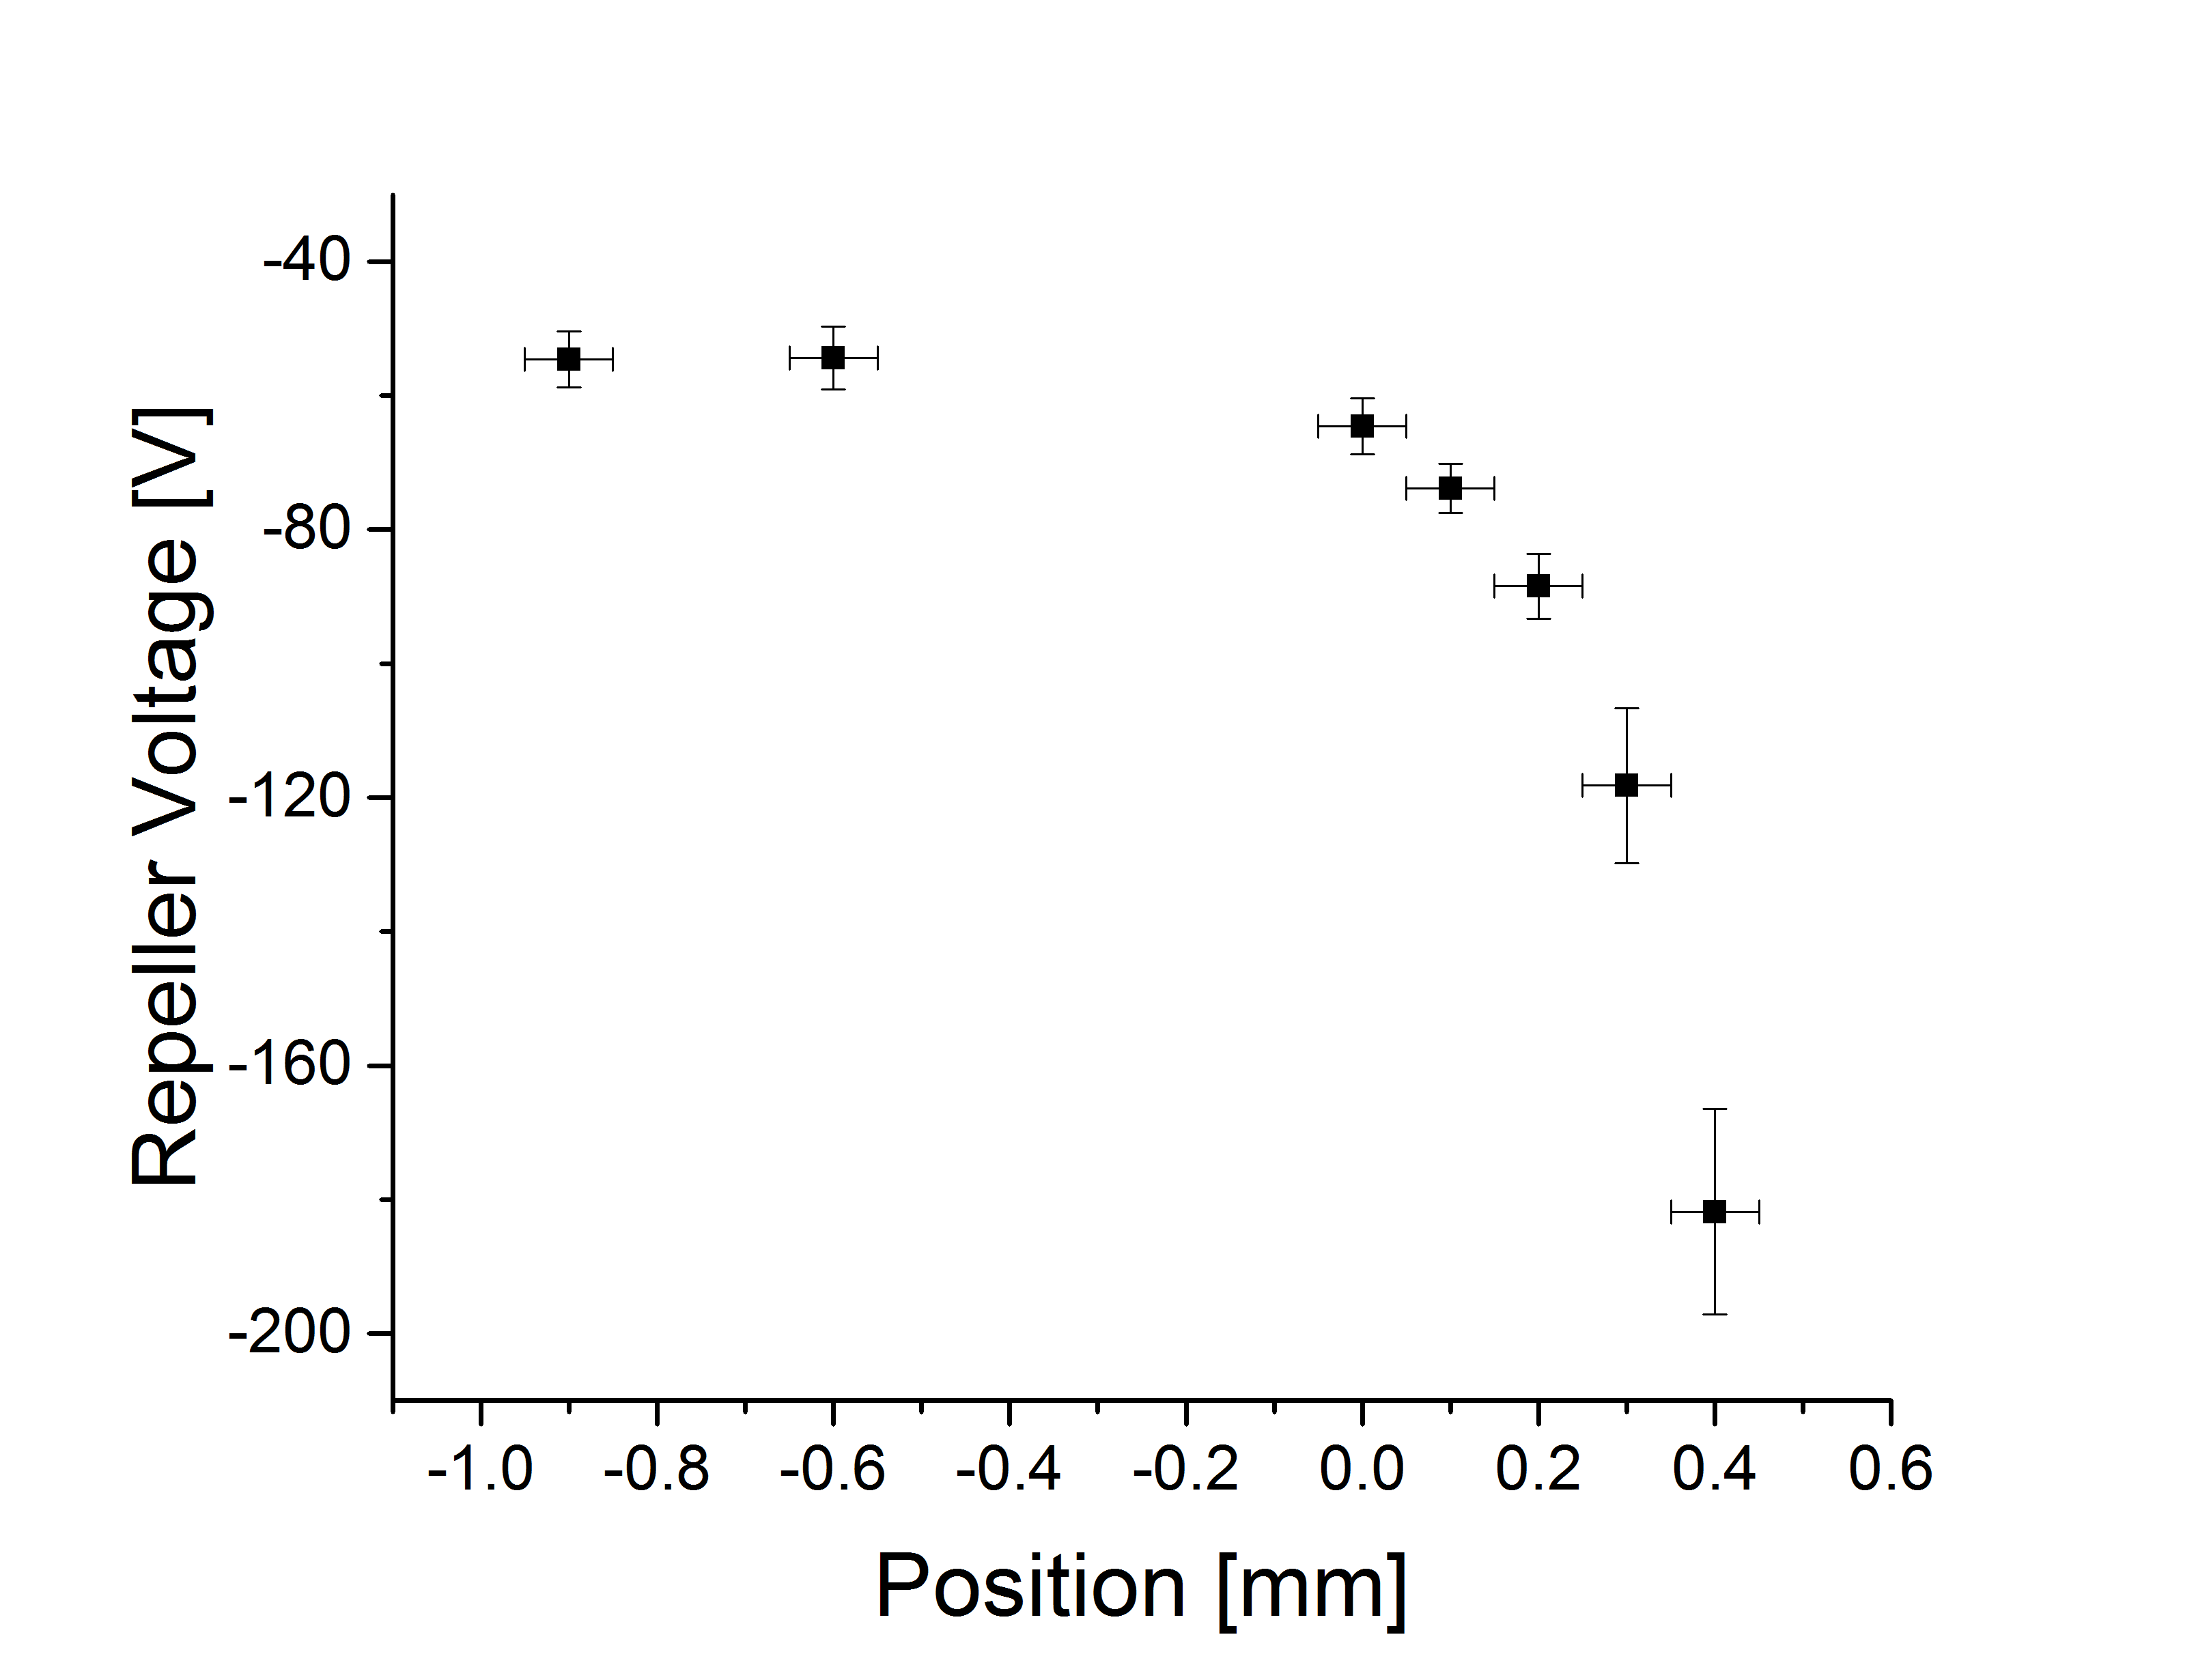
\includegraphics[width= 0.95\textwidth]{Messungen/SimRepPosU.png}
		\end{subfigure}
		\begin{subfigure}{0.47\textwidth}
			\centering
			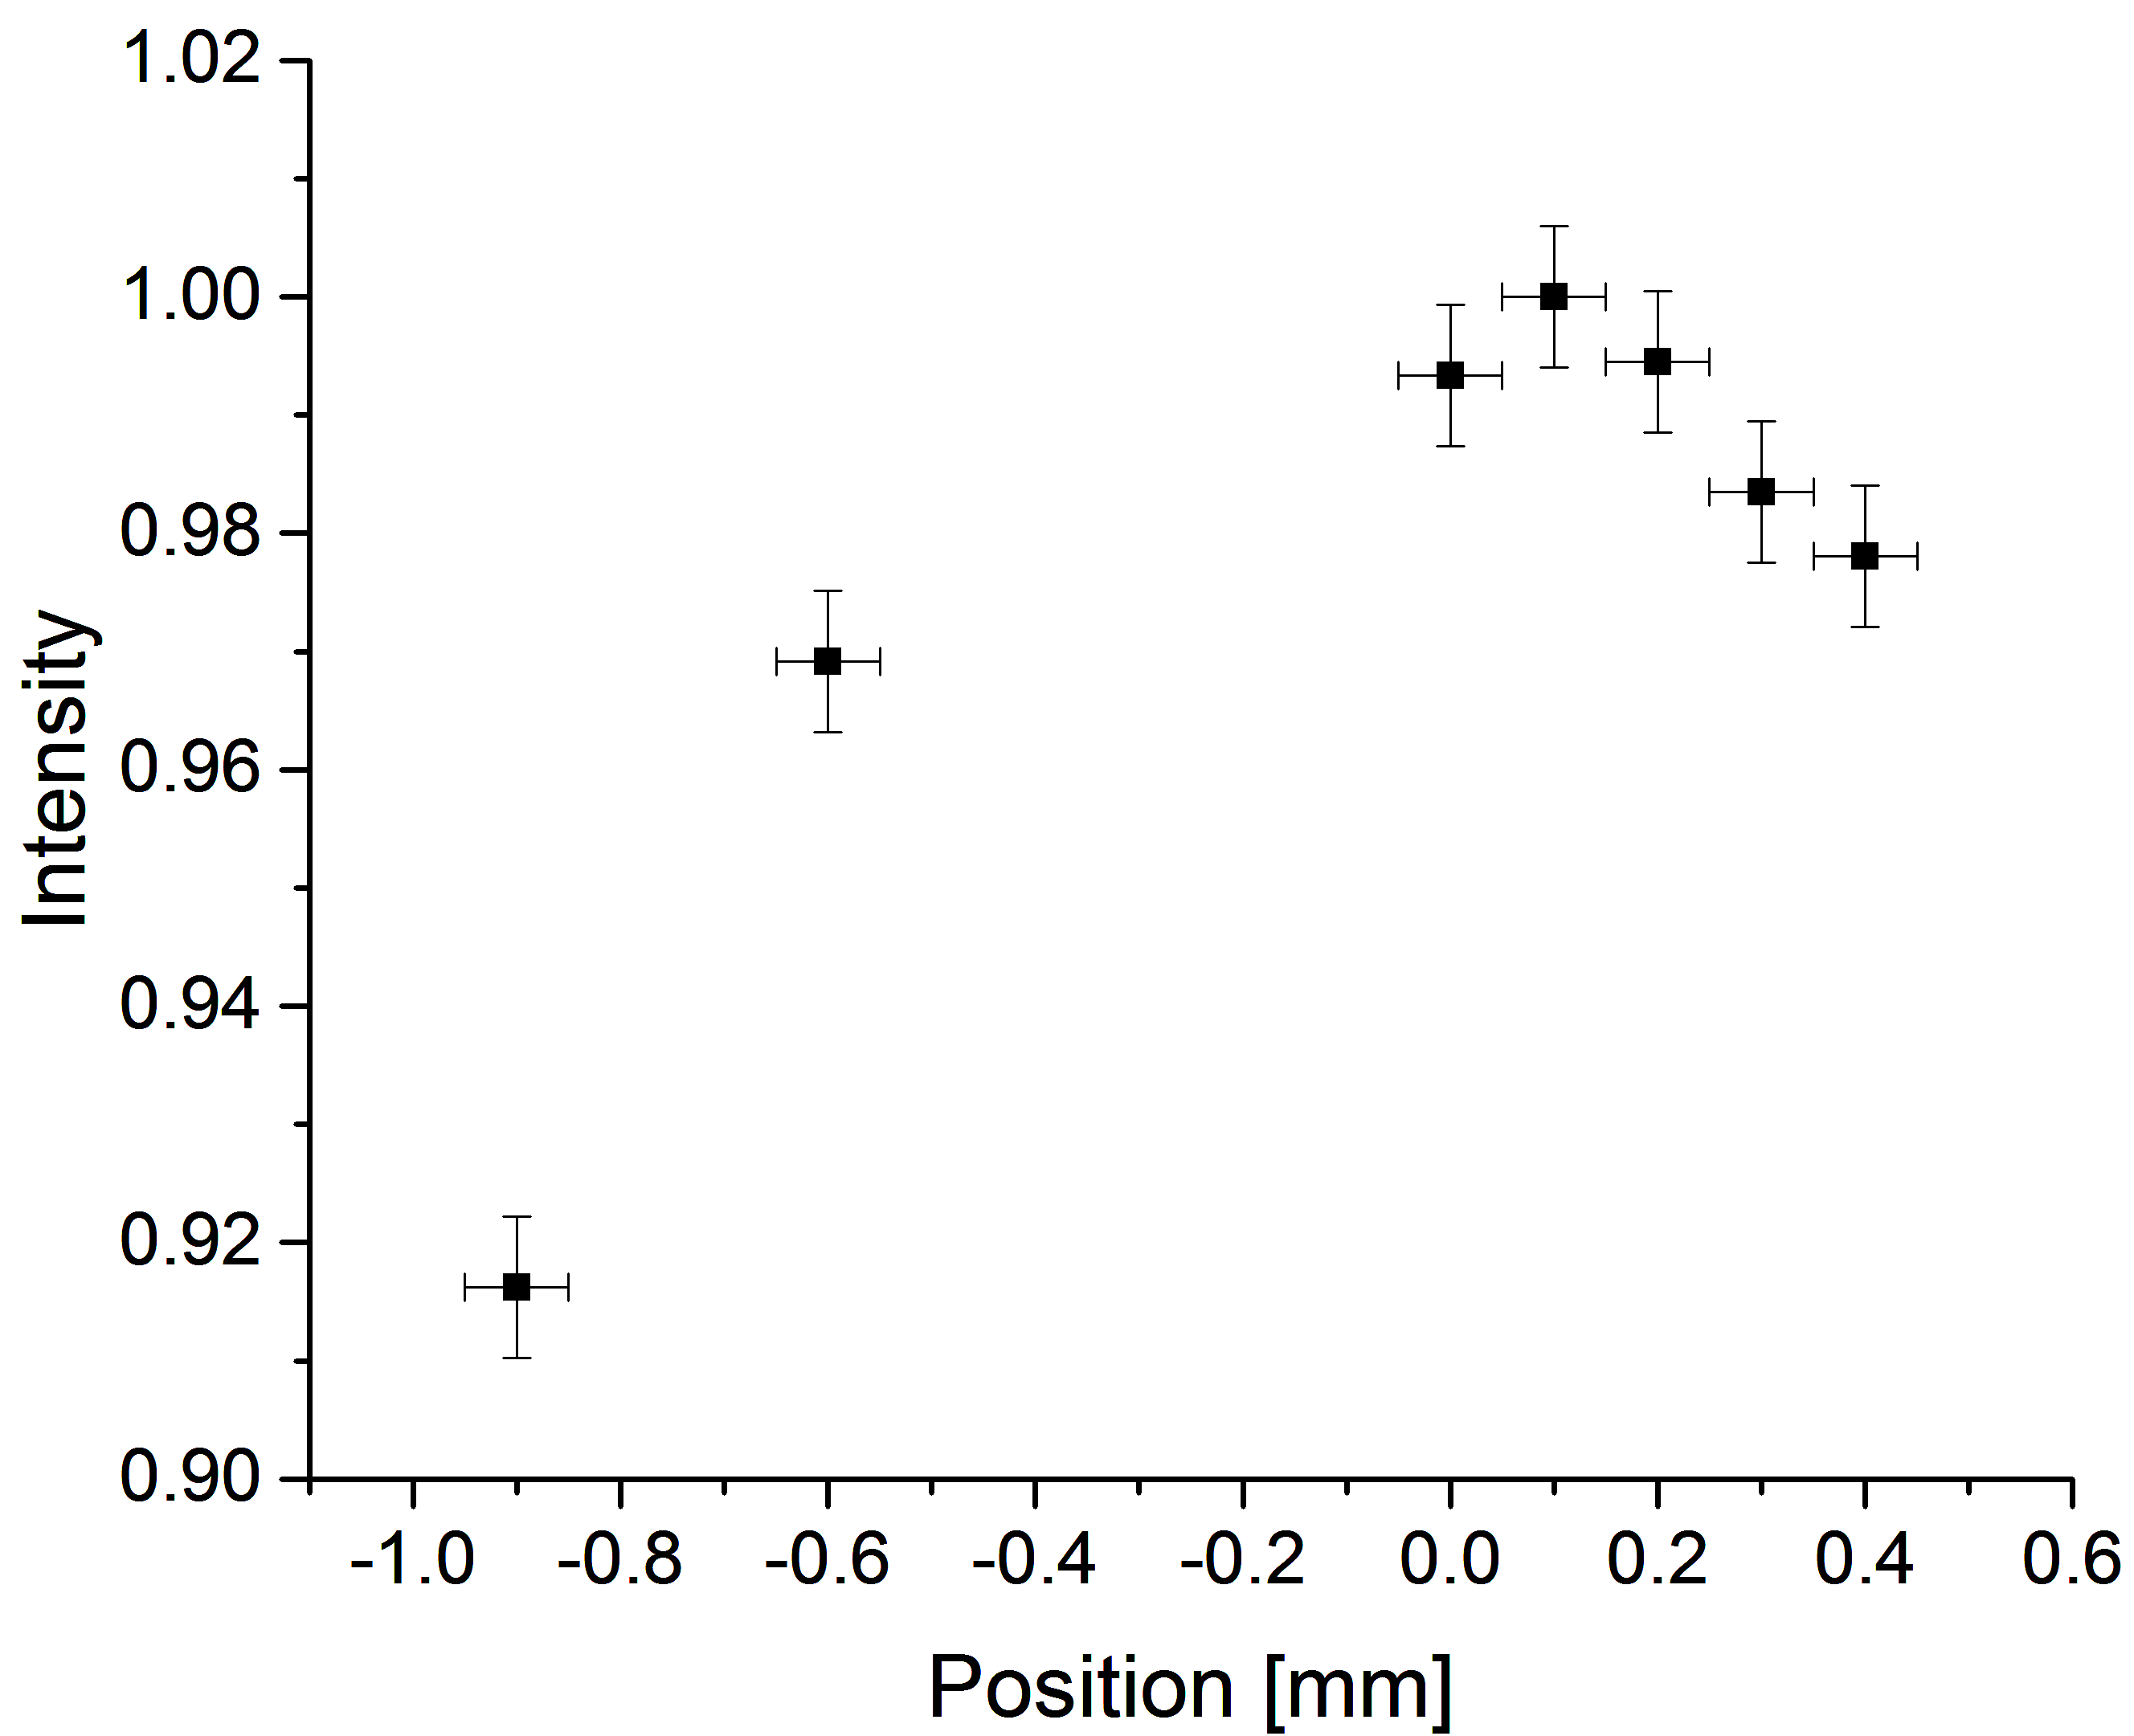
\includegraphics[width= 0.95\textwidth]{Messungen/SimRepPosImax.png}
		\end{subfigure}
		\caption{Left: The filament repeller voltage to reach the maximum electron intensity over the volume of the neutral particles. Right: Electron intensity normed on the intensity at position 0.} % Noch Graphik wie Intensität bei den versch. Pos abfällt.
		\label{fig:ExpSimRep}
	\end{figure}


%-------------------------------------------------------------------------------------
	\subsection{Pulser}
	
	% Einfach Resultate von Tests einfügen. Die Verbreiterung erst erwähnen, wenn man mehr Daten hat oder man klarer weiss, woher die Verbreiterung kommt/ was sie auslöst. ???
	% Pulsertests, Messungen, Simulationsresultate
	% Two different pulsers properties, pulse shape. Tests with different gases. Massresolution, Intensity relation?, SNR? Are these two properties correlated? Noch mit Peter anschauen. Ar sieht in allen 4 Fällen etwas komisch aus. Higher signal intensity -> higher SNR.
	% Achsenskalierung anschauen von Areagraphik. Wenn das geklärt ist, evt. in Matlab schreiben. Zusätzliches Skript für diese Graphiken, Stefans Vorlagen anschauen. Die signal intensity lässt sich nicht einfach in Druck umrechnen. Zu viele unbekannte Komponenten -> a.u. oder # e-/ns angeben.
	
	
	
	\subsection{Detector Tests}
	% Plot off the gain curves of the detector in its different states. flat, folded, folded in the wolfram copper shealding. If there should be any time, redo the errorcalculation correctly (error from the calculation of the area under the peak = charge and of the conversion factor when using a different discriminator level).
	% Measuring settings. Turn the drift voltage up to -2.5 kV and then slowly increase the anode voltage to the value you want to measure. The gain is calculated with the software by doing a Simpson 3/8 integration of the peak = Q. (Look in the lab book for the proper calculation)
	
	
%----------------------------------------------------------------------------------------
	\subsection{Ionoptics}
	% Ionenoptitktests. PFM
	
	
	
	
	
	
	
	
	